% Import default values & document settings
% Layout settings
\newcommand{\FIITdefaultFontSize}[0] {12pt}
\setcounter{secnumdepth}{3}
\setcounter{tocdepth}{3}

% Language settings
% \newcommand{\FIITlanguage}[0] {slovak}
\newcommand{\FIITlanguage}[0] {slovak,english}
\def\FIITlagEN{}

% Global texts
\newcommand{\FIITuniversity}[0] {Slovak University of Technology in Bratislava}
\newcommand{\FIITuniversitySK}[0] {Slovenská technická univerzita v Bratislave}
\newcommand{\FIITfaculty}[0] {Faculty of informatics and information technologies}
\newcommand{\FIITfacultySK}[0] {Fakulta informatiky a informačných technológií}
\newcommand{\FIITthesis}[0] {Bachelor's thesis}
\newcommand{\FIITthesisSK}[0] {Bakalárska práca}
\newcommand{\FIITtitle}[0] {Practical usage of Zero-knowledge in different use-cases in blockchains}
\newcommand{\FIITtitleSK}[0] {Praktické využitie dôkazov s nulovým vedomím v rôznych prípadoch použitia v blockchainoch}
\newcommand{\FIITauthor}[0] {Lukáš Častven}
\newcommand{\FIITsupervisor}[0] {Ing. Kristián Košťál PhD.}
\newcommand{\FIITevidenceNumber}[0] {FIIT-16768-116160}
\newcommand{\FIITdate}[0] {May 2024}
\newcommand{\FIITdateSK}[0] {May 2024}
\newcommand{\FIITstudyProgram}[0] {Informatics}
\newcommand{\FIITstudyProgramSK}[0] {Informatika}
\newcommand{\FIITstudyField}[0] {Computer Science}
\newcommand{\FIITdegreeCourseSK}[0] {9.2.1 Informatika}
\newcommand{\FIITinstitute}[0] {Institute of Computer Engineering and Applied Informatics}
\newcommand{\FIITinstituteSK}[0] {Ústav počítačového inžinierstva a aplikovanej informatiky}
\newcommand{\FIITsignPlace}[0] {In Bratislava, }
\newcommand{\FIITsignPlaceSK}[0] {V Bratislave, }
\newcommand{\FIITsignDate}[0] {25.12.2023}
\newcommand{\FIITArchiveName}[0] {BP\_LukasCastven.zip}


% Setup document
\documentclass[\FIITdefaultFontSize,a4paper,twoside,openright,\FIITlanguage]{book}

% Load all necessary packages
\usepackage[final]{pdfpages}
\usepackage[utf8]{inputenc}
\usepackage[T1]{fontenc}
\usepackage[\FIITlanguage]{babel}
\usepackage[a4paper]{geometry}
\usepackage[
  left = \glqq,% 
  right = \grqq,% 
  leftsub = \glq,% 
  rightsub = \grq%
]{dirtytalk}
\usepackage[parfill]{parskip}
\usepackage{enumitem}
\usepackage{calc}
\usepackage{graphicx}
\usepackage{float}
\usepackage{csquotes}
\usepackage{longtable}
\usepackage{setspace}
\usepackage{tabularx}
\usepackage{fancyhdr}
\usepackage[backend=bibtex,sorting=none]{biblatex}
\usepackage{listing}
\usepackage{lscape}
\usepackage{afterpage}
\usepackage{hyperref}
\usepackage{bera}
\usepackage{listings}
\usepackage{xcolor}
\usepackage{lipsum}
\usepackage{minted}
\usepackage{tikz}
\usepackage{tocloft}

% Remove unnecessary gap between paragraph if large figure is inserted after them
\raggedbottom

% lscape.sty Produce landscape pages in a (mainly) portrait document.
\usepackage{lscape}

% Custom commands
\newcommand{\signaturespace}[2]{
  % #1 = width of the dotted line
  % #2 = legend
  \begingroup
  \renewcommand{\arraystretch}{0}
  \begin{tabular}[t]{cc}
    \hspace*{0pt}
    \cleaders\hbox{\kern.6pt.\kern.6pt}\hskip#1\relax
    \hspace*{0pt}
    \\[0.5cm]
    #2
  \end{tabular}
  \endgroup
}

\newcommand{\emptypage}{\newpage
  \thispagestyle{empty}
  \mbox{}
  \newpage}

% openright does not work :(
\let\tmp\oddsidemargin
\let\oddsidemargin\evensidemargin
\let\evensidemargin\tmp
\reversemarginpar


% Setup bibliography
\bibliography{bibliography}

% Page design
\pagestyle{fancy}
\lhead{\nouppercase{\leftmark}}
\chead{}
\rhead{}
\lfoot{}
\cfoot{\thepage}
\rfoot{}

\begin{document}

% Initialize document
% Layout
\setstretch{1.5}

% Bibliography
\ifx\FIITlagEN\undefined
  \defbibheading{references}[Zoznam použitej literatúry]{
    \chapter*{#1}
    \addcontentsline{toc}{chapter}{#1}
    \markboth{#1}{#1}
  }
  \defbibheading{referencessec}[Zoznam použitej literatúry]{
    \section*{#1}
    \markboth{#1}{#1}
  }
\else
  \defbibheading{references}[References]{
    \chapter*{#1}
    \addcontentsline{toc}{chapter}{#1}
    \markboth{#1}{#1}
  }
  \defbibheading{referencessec}[References]{
    \section*{#1}
    \markboth{#1}{#1}
  }
\fi

% Syntax highlighting
\setminted[]{linenos,tabsize=2,breaklines}
\colorlet{punct}{red!60!black}
\definecolor{background}{HTML}{EEEEEE}
\definecolor{delim}{RGB}{20,105,176}
\colorlet{numb}{magenta!60!black}

% Text highlighting
\makeatletter
\newenvironment{btHighlight}[1][]
{\begingroup\tikzset{bt@Highlight@par/.style={#1}}\begin{lrbox}{\@tempboxa}}
    {\end{lrbox}\bt@HL@box[bt@Highlight@par]{\@tempboxa}\endgroup}

\newcommand\btHL[1][]{%
  \begin{btHighlight}[#1]\bgroup\aftergroup\bt@HL@endenv%
    }
    \def\bt@HL@endenv{%
  \end{btHighlight}%   
  \egroup
}
\newcommand{\bt@HL@box}[2][]{%
  \tikz[#1]{%
    \pgfpathrectangle{\pgfpoint{1pt}{0pt}}{\pgfpoint{\wd #2}{\ht #2}}%
    \pgfusepath{use as bounding box}%
    \node[anchor=base west, fill=black!10,outer sep=0pt,inner xsep=1pt, inner ysep=-2pt, rounded corners=3pt, minimum height=\ht\strutbox+1pt,#1]{\raisebox{1pt}{\strut}\strut\usebox{#2}};
  }%
}
\makeatother

% TODO https://www.fiit.stuba.sk/buxus/docs/organizacia_studia/pokyny/ZP-clenenie-pokyny_2022.pdf
%   https://www.fiit.stuba.sk/studium/bakalarsky-projekt/bp.html?page_id=1862
% Cover & title page
% Cover page
	\begin{center}
\thispagestyle{empty}
\ifx\FIITlagEN\undefined
{\Large \FIITuniversitySK}
\else
{\Large \FIITuniversity}
\fi
\par\end{center}{\Large \par}

\begin{center}
\ifx\FIITlagEN\undefined
{\Large \FIITfacultySK}
\else
{\Large \FIITfaculty}
\fi
\par\end{center}{\Large \par}

\smallskip{}

\begin{center}
\ifx\FIITlagEN\undefined
Evidenčné číslo: \FIITevidenceNumber
\else
Reg. No.: \FIITevidenceNumber
\fi
\par\end{center}
\vfill{}

\begin{center}
\textbf{\Large \FIITauthor}
\par\end{center}{\Large \par}

\medskip{}


\begin{center}
\ifx\FIITlagEN\undefined
\textbf{\LARGE \FIITtitleSK}
\else
\textbf{\LARGE \FIITtitle}
\fi
\par\end{center}{\huge \par}

\medskip{}


\begin{center}

\ifx\FIITlagEN\undefined
{\Large \FIITthesisSK}
\else
{\Large \FIITthesis}
\fi
\par\end{center}{\Large \par}

\vfill{}

\ifx\FIITlagEN\undefined
Vedúci záverečnej práce: \FIITsupervisor
\else
Thesis supervisor: \FIITsupervisor
\fi

\medskip{}

\ifx\FIITlagEN\undefined
\FIITdateSK
\else
\FIITdate
\fi

\pagenumbering{roman}
\emptypage





% Thesis title page
	\begin{center}
\thispagestyle{empty}
\ifx\FIITlagEN\undefined
{\Large \FIITuniversitySK}
\else
{\Large \FIITuniversity}
\fi
\par\end{center}{\Large \par}

\begin{center}
\ifx\FIITlagEN\undefined
{\Large \FIITfacultySK}
\else
{\Large \FIITfaculty}
\fi
\par\end{center}{\Large \par}

\smallskip{}

\begin{center}
\ifx\FIITlagEN\undefined
Evidenčné číslo: \FIITevidenceNumber
\else
Reg. No.: \FIITevidenceNumber
\fi
\par\end{center}
\vfill{}

\begin{center}
\textbf{\Large \FIITauthor}
\par\end{center}{\Large \par}

\medskip{}


\begin{center}
\ifx\FIITlagEN\undefined
\textbf{\LARGE \FIITtitleSK}
\else
\textbf{\LARGE \FIITtitle}
\fi
\par\end{center}{\huge \par}

\medskip{}


\begin{center}

\ifx\FIITlagEN\undefined
{\Large \FIITthesisSK}
\else
{\Large \FIITthesis}
\fi
\par\end{center}{\Large \par}

\vfill{}

\ifx\FIITlagEN\undefined
Študijný program: \FIITstudyProgramSK

Študijný odbor: \FIITdegreeCourseSK

Školiace pracovisko: \FIITinstituteSK

Vedúci záverečnej práce: \FIITsupervisor
\else
Study programme: \FIITstudyProgram

Study field: \FIITstudyField

Training workplace: \FIITinstitute

Thesis supervisor: \FIITsupervisor
\fi

\medskip{}

\ifx\FIITlagEN\undefined
\FIITdateSK
\else
\FIITdate
\fi

\emptypage


% Thesis assignment
\newpage
\thispagestyle{empty}
\begin{center}
    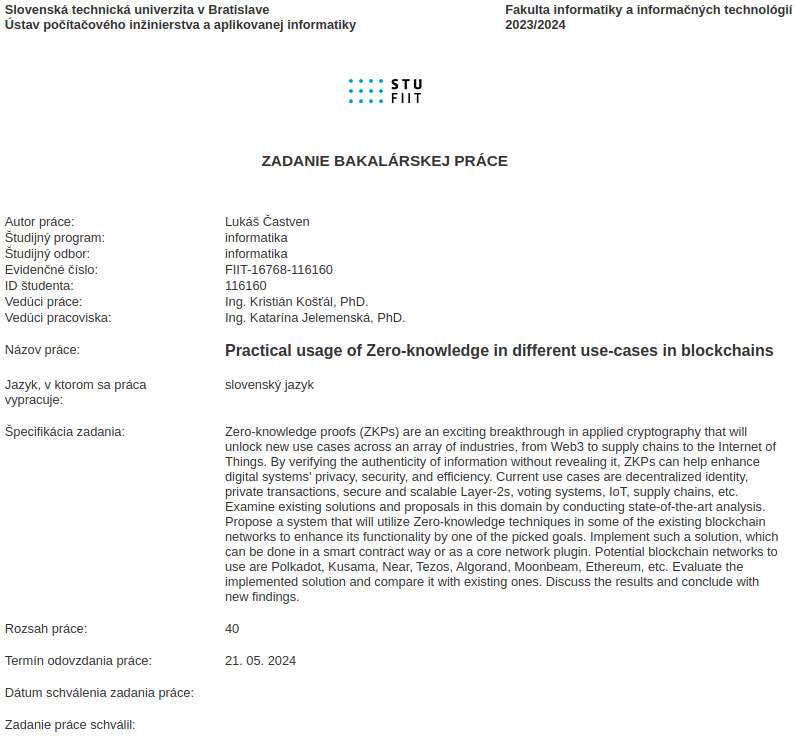
\includegraphics[scale=0.65]{assets/assignment.png}
\end{center}
\newpage

% Declaration of honor
% TODO
% \thispagestyle{empty}

\vspace*{\fill}

\ifx\FIITlagEN\undefined
\section*{Čestné prehlásenie}
\else
\section*{Declaration of honor}
\fi

\lipsum[3]

\ifx\FIITlagEN\undefined
\FIITsignPlaceSK \FIITsignDate
\else
\FIITsignPlace \FIITsignDate
\fi
\hspace*{\fill} \signaturespace{5cm}{\FIITauthor}

\emptypage

% Acknowledgements
% TODO
% \thispagestyle{empty}

\vspace*{\fill}

\ifx\FIITlagEN\undefined
\section*{Poďakovanie}
\else
\section*{Special thanks}
\fi

\lipsum[1]

\emptypage

% Annotation
% Annotation in Slovak
\thispagestyle{empty}

\vspace*{\fill}

\section*{Anotácia}

\begin{minipage}[t]{1\columnwidth}
    \FIITuniversitySK

    \FIITfacultySK

    Študijný program: \FIITstudyProgramSK\\

    Autor: \FIITauthor

    \FIITthesisSK: \FIITtitleSK

    Vedúci projektu: \FIITsupervisor

    \FIITdateSK
\end{minipage}

\bigskip{}

Bakalárska práca skúma aplikáciu dôkazov s nulovým vedomím (ZKPs) v
blockchaine. Dôkazy s nulovým vedomím sú kryptografická metóda, ktorá
umožňuje overenie dát bez odhalenia samotných dát, čo je ideálne pre bezpečné
a súkromné aplikácie v blockchainoch. Táto práca je zameraná na návrh
a implementáciu konceptu schémy tajných adries s použitím ZKPs. Táto schéma
umožňuje odosielateľom odvodiť tajnú adresu z verejných údajov príjemcu.
Iba príjemca má kontrolu nad touto adresou, a zaroveň neodhaľuje žiadne informácie
o tom, kto príjemca je.

Výskum zahŕňa analýzu kryptografických princípov za ZKPs, nasledovanú
vysvetlením návrhu schémy tajných adries a jej integráciou do blockchainu Ethereum.

Táto práca prispieva do oblasti ukázaním, ako možno využiť ZKPs v blockchaine
na riešenie problémov súkromia, ponúkajúc riešenie vo forme konceptuálnej
implementácie schémy tajných adries s použitím ZKPs.

\newpage{}\thispagestyle{empty}\medskip{}

\emptypage

% Annotation in English
\thispagestyle{empty}

\vspace*{\fill}

\section*{Annotation}

\begin{minipage}[t]{1\columnwidth}
    \FIITuniversity

    \FIITfaculty

    Degree Course: \FIITstudyProgram\\

    Author: \FIITauthor

    \FIITthesis: \FIITtitle

    Supervisor: \FIITsupervisor

    \FIITdate
\end{minipage}

\bigskip{}

This bachelor's thesis investigates the application of Zero Knowledge Proofs
(ZKPs) in blockchains. Zero Knowledge Proofs are a cryptographic
method which enables the validation of data without revealing the
data itself, making it ideal for secure and private applications in
blockchain networks. The focus of this thesis is the design and implementation
of a proof of concept Stealth Address scheme using ZKPs. This scheme allows any sender to
derive a stealth address from recipients public data. Only the recipient has
control over this address, yet it does not leak any information about who the
recipient is.

The research includes an analysis of the cryptographic principles behind
ZKPs, followed by an explanation of the Stealth Address scheme's design and
its integration into a an Ethereum blockchain.

This thesis contributes to the field by showcasing how ZKPs can be utilized
in blockchain to address privacy concerns, offering a solution in the form of
a proof of concept  implementation of Stealth Address scheme using ZKPs.

\newpage{}\thispagestyle{empty}

\emptypage


% Table of contents
\ifx\FIITlagEN\undefined
    \renewcommand{\contentsname}{Obsah}
\else
    \renewcommand{\contentsname}{Table of contents}
\fi
\tableofcontents{}

% List of figures
\listoffigures

% List of tables
%\listoftables

% List of abbreviations
\thispagestyle{plain}

\ifx\FIITlagEN\undefined
    \section*{\Huge Zoznam použitých skratiek}
    \markboth{Zoznam použitých skratiek}{Zoznam použitých skratiek}
\else
    \section*{\Huge List of abbreviations used}
    \markboth{List of abbreviations used}{List of abbreviations used}
\fi
\vskip 1cm

\begin{tabular}{ >{\bfseries}m{2cm} m{10cm} }
	AC  & Arithmetic Circuit       	\\
	ERC & Ethereum Request for Comments \\
	EVM & Ethereum Virtual Machine 	\\
	SNARK & Succinct Non-interactive Argument of Knowledge \\
	R1CS & Rank-1 Constraint System \\
	ZK  & Zero Knowledge           	\\
	ZKP & Zero Knowledge Proof
    % API		& Application Programming Interface \\
    % AWS		& Amazon Web Services \\
    % CNAME	& Canonical Name record \\
    % CSV		& Comma-Separated Values \\
    % DNS		& Domain Name System \\
    % HTTP	& Hyper-Text Transfer Protocol \\
    % ICANN	& Internet Corporation for Assigned Names and Numbers \\
    % IMAP	& Internet Message Access Protocol \\
    % IP		& Internet Protocol \\
    % JSON	& JavaScript Object Notation \\
    % MD5		& Message-Digest algorithm, version 5 \\
    % MSSQL	& Microsoft SQL \\
    % MX		& Mail Exchanger record \\
    % MySQL	& Maria SQL  \\
    % NS		& Name Server \\
    % OS		& Operating System \\
    % POP3    & Post Office Protocol, version 3\\
    % REST    & Representational state transfer \\
    % S3		& Amazon Simple Storage Service \\
    % SHA1	& Secure Hash Algorithm 1 \\
    % SMTP	& Simple Mail Transfer Protocol \\
    % SQL		& Structured Query Language \\
    % SRV		& Service record
\end{tabular}

\begin{tabular}{ >{\bfseries}m{2cm} m{10cm} }
    % TLD		& Top-Level Domain \\
    % TLS     & Transport Layer Security \\
    % URL		& Unified Resource Locator \\
    % XML		& Extensible Markup Language  
\end{tabular}

\emptypage


% Enable page numbering
\pagenumbering{arabic}

% Begin references segment
\begin{refsegment}
    \chapter{Introduction}

Zero Knowledge Proofs (ZKPs) are a powerful cryptography primitive. They allow
for the verification of a statement's truth without disclosing or in any way revealing
the actual content of the statement. This characteristic is crucial for
maintaining trust between parties while also preserving privacy.

The concept of ZKPs was first introduced in a 1989 research paper, "The
Knowledge Complexity of Interactive Proof Systems."\cite{Goldwasser1989}.
This work describes how in traditional proofs, such as demonstrating a graph
is Hamiltonian, more information is typically revealed than just the truth of
the theorem. This paper develops a computational complexity theory focusing
on the knowledge part within a proof. It introduces zero knowledge proofs,
a novel concept where proofs only confirm the correctness of a proposition
without exposing any extra knowledge. The paper focuses on interactive
proofs, where a dialogue between a prover and a verifier occurs. In these
interactive proofs, the prover aims to convince the verifier about the truth
of a private statement, with a very small probability of error. This
interaction is pivotal in ZKPs, as it allows for the verification of a
statement's truth without revealing the actual information or knowledge
behind the statement, maintaining the principle of conveying no
knowledge beyond the proposition's correctness.

This thesis extends the application of ZKPs to the concept of stealth
addresses in blockchain, as outlined in Vitalik Buterin's article "An
Incomplete Guide to Stealth Addresses."\cite{ButerinIncompleteGuide}.
Stealth addresses are critical for privacy on blockchains, allowing assets to
be transferred without revealing the recipient's identity and making
it difficult to link transactions to specific individuals.

Stealth addresses allow a sender (Alice) to transfer assets to a receiver (Bob) without
publicly revealing Bob's identity. To achieve this, Bob
must first provide a public meta stealth address generation data. This data
has different structure based on the underlying stealth address generation
schema. From this data Alice computes a new stealth address that only Bob can
control, and sends the assets to that newly generated address. Bob can then
access these assets from another address, only by providing a ZKP of given
address ownership.



    \chapter{Analysis}

The analysis section of the thesis starts with demonstration of interactive
proofs with goal to build up intuition behind interactive proofs \cite{Goldwasser1989,youtubeMOOCLecture1}.
This section explains how Alice attempts to prove to Bob that she knows an
algorithm, with which she computes some pair (N, y), such that this pair is
part of the quadratic residue language QR. Specifically, Alice needs to
convince Bob that there exists an x, such that y equals x squared modulo N,
effectively placing the pair (N, y) within the QR language, which includes all
pairs where y is a quadratic residue of N.

The analysis section continues by highlighting a practical limitation of
interactive proofs in real world cryptography. It notes that for Alice to
prove something to multiple parties, she would need to engage in separate
interactions with each one. This approach is not scalable and becomes
impractical for widespread verification needs. However, the thesis introduces
the Fiat-Shamir transform \cite{Fiat}, a significant breakthrough that addresses this
issue. This transform allows for converting the interactive proof into a
non-interactive format by processing the interaction transcript, making the
proof more practical and scalable for real-world cryptographic applications.

While in theory any NP statement \cite{goldreich1991proofs} can be proven using
interactive proofs, practical implementation requires specific definition and
encoding of the statement. There are two main models of general computation,
those are circuits and turing machines. To trace the computation of a turing
machine, the representation needs to somehow handle memory and thus would accrue
more complexity than if a circuit is used. To represent a statement as a
circuit, an arithmetic circuit, a computation model composed of addition and
multiplication operations, is used. This circuit encodes the statement into a
form suitable for "zk-ifying", enabling the application of interactive proofs
to a broader range of practical scenarios.

The analysis section then explores SNARKs (Succinct Non-interactive ARguments
of Knowledge), which are most commonly used ZKP system today. They are succinct,
meaning that the size of the proof is small and have a relatively fast verification
time.

The final part of the analysis examines how ZKP systems such as SNARKs enable
the creation of a stealth address scheme that upholds privacy and security.
This section assesses how these systems fulfill the necessary properties for a
stealth address scheme, focusing on their ability to ensure transaction
confidentiality while maintaining the anonymity of the recipient's identity.

\section{Proof of quadratic residuosity}

This first part focuses on demonstrating an interactive proof where Alice aims
to prove to Bob that she knows an algorithm, which computes some pair (N, y),
such that this pair is part of the quadratic residue language QR \cite{Goldwasser1989}.
QR is defined as:

\[QR = \lbrace(N, y): \exists x, y \equiv x^2 \pmod{N}\rbrace\]

\begin{figure}[h!]
    \centering
    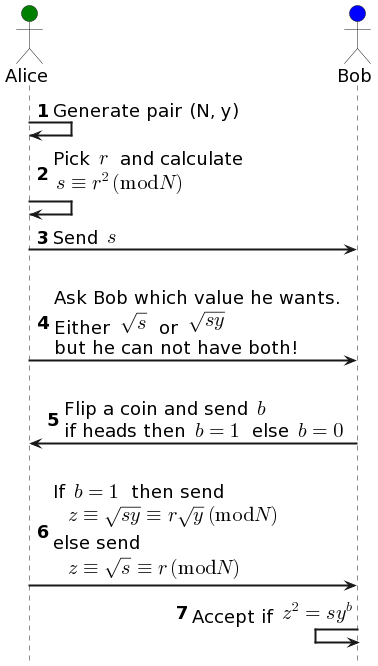
\includegraphics[scale=0.6]{assets/images/qr_ip.png}
    \caption{Interactive proof of language QR}
    \label{fig:qr_ip}
    \vspace{0.5cm}
\end{figure}

\begin{enumerate}
    \item Alice generates pair (N, y)
    \item Alice picks a random $r$ such that $1 \leq r \leq N$ and $\gcd(r, N) = 1$
          and calculates $s \equiv r^2 \pmod{N}$
    \item Alice sends Bob $s$
    \item Alice asks Bob which value he wants. Either $\sqrt{s}$ or $\sqrt{sy}$, but he can not have both!
    \item Bob flips a coin and sends $b$ such that if coin landed on heads $b = 1$ else $b = 0$
    \item If $b = 1$ Alice sends to Bob $z \equiv \sqrt{sy} \equiv r \sqrt{y} \pmod{N}$ else she sends $z \equiv \sqrt{s} \equiv r \pmod{N}$
    \item Bob accepts if $z^2 = sy^b$
\end{enumerate}

If Alice was a cheating prover, and she didn't have the algorithm for
generating pairs from QR, then the probability that Bob's coin toss favors
Alice is one half. With one half probability Bob would ask cheating prover
Alice to give him the equation she can not solve, because if the prover is
cheating, she can not find the $\sqrt{s}$ and $\sqrt{sy}$. If she could,
that would mean that she is not cheating.

If the Alice's claim is true, Bob will accept. If Alice is not honest, and
cheats, all verifiers will not accept with probability $P(Accept) = 0.5$.
But this probability may not be satisfying enough. To make the probability
that Alice is cheating smaller, Bob and Alice can start the interaction once
again. This would lead to $P(Accept) = (0.5)^2$. They can redo the process
as many times as they wish, resulting in $P(Accept) = (0.5)^k$ where $k$
is how many different interactions they performed.

Thanks to the randomness of the coin toss, there are $2^k$ possibilities how
the interaction can go. Since Alice can't reliably predict what the random
coin toss will yield, she must be ready to provide both equations. Thus Bob is
convinced, that Alice isn't cheating, with probability $P(Accept) = (0.5)^k$,
and can accept the proof.

\section{Non-interactive proofs}

Interactive proofs require Alice to engage in a unique interaction with each
individual verifier, which is not scalable or feasible for widespread
application. Many ZKP protocols only require from the verifier a random input
(for instance, a coin toss). Protocols, in which the verifier's role is
generating some randomness and making it public are called public coin protocols \cite{Babai1988,Goldwasser1986}.
The paper "How To Prove Yourself: Practical Solutions to Identification and
Signature Problems"\cite{Fiat} by Fiat and Shamir demonstrates how these
interactive public coin protocols can be efficiently transformed into
non-interactive ones, offering a more scalable and practical solution for ZKPs.

To transform a interactive public coin protocol into a non-interactive,
Alice uses a random oracle which can provide a random coin toss based on some
input. In practice the source of randomness of the random oracle is a
cryptographic hash function, such as SHA256. Instead of sending messages back
and forth between Alice and Bob, Alice provides to Bob a transformed
transcript of the interaction. Since Bob's role in this interaction would only
be generating random coin toss, Alice can in advance query the random oracle
for this random value, and supply the message as an input to the query. The
transcript string would look like this $(msg1, query(msg1), msg2, ...)$, where $query$ is
the output from random oracle. This string and the public input of the proof
can then be published and anybody, not just Bob, can validate this proof
on their own.

In scenario when Alice sends only two messages and requires one random coin toss
from Bob,
\begin{figure}[h]
    \centering
    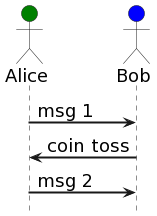
\includegraphics[scale=0.6]{assets/images/interactive_coin.png}
    \caption{Interactive public coin proof}
    \label{fig:interactive_coin}
    \vspace{0.5cm}
\end{figure}
Bob at the end can compute the validity of the proof from Alice with
$validate(public\:input\:x,\:msg1,\:coin\:toss,\:msg2) = accept/reject$

Then after applying Fiat-Shamir transform, Alice only sends one message with
the transcript string,
\begin{figure}[h]
    \centering
    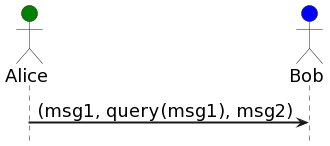
\includegraphics[scale=0.6]{assets/images/non_interactive_coin.png}
    \caption{Non-interactive public coin proof}
    \label{fig:non_interactive_coin}
    \vspace{0.5cm}
\end{figure}
and Bob can compute the validity of the proof like this
$validate(public\:input\:x,\:msg1,\:query(msg1),\:msg2) = accept/reject$.

\section{Arithmetic circuit}

The computation model used to create ZKPs is an arithmetic circuit in a
finite field $\mathbb{F}_p$. The arithmetic circuit is a function which takes
$n$ elements from field $\mathbb{F}_p$ and returns one element from that field.

\[AC: \mathbb{F}^n \rightarrow F \]

The $AC$ can be represented as a directed acyclic graph, or a polynomial. For
example, polynomial $x_1x_2 + (x_2 + x_3)^2$ represents the same circuit as this
directed acyclic graph

\begin{figure}[h]
    \centering
    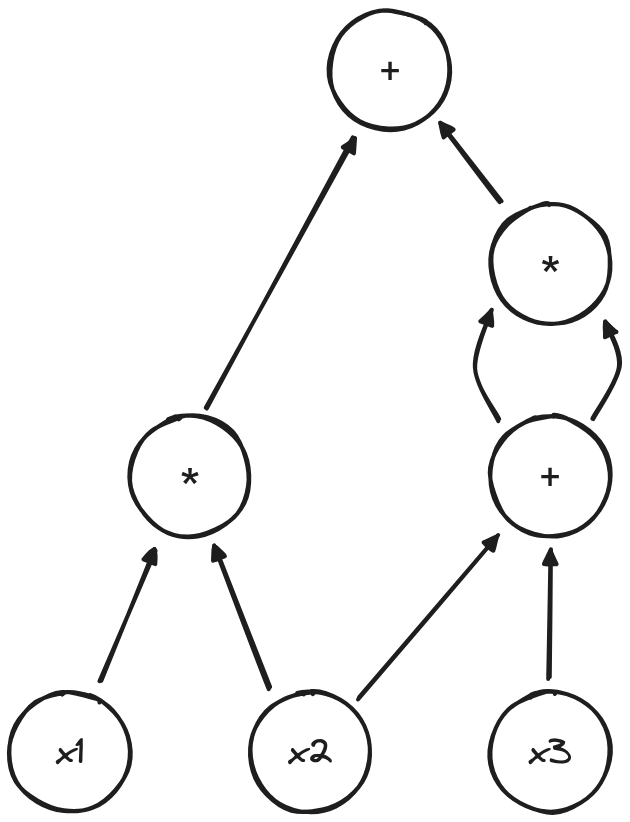
\includegraphics[scale=0.25]{assets/images/dag_example.png}
    \caption{Graph representation of arithmetic circuit}
    \label{fig:dag_example}
    \vspace{0.5cm}
\end{figure}

Another representation of a arithmetic circuits is called a Rank 1 Constraint
System (R1CS). R1CS is a system of equations of a form $\alpha \times \beta = \gamma$,
where $\alpha, \beta, \gamma$ are affine combinations of variables $w$ and $x$,
where $w$ is a witness (private inputs) and $x$ is a public inputs.

These are some examples of R1CS equations:
\begin{displaymath}
    \begin{array}{l}
        (w_1 + x_3) \times (w_2 - x_1 + 1) = w_3 \\
        w_1 \times w_1 = x_1                     \\
        w_1 \times x_2 = w_3
    \end{array}
\end{displaymath}

And here is an example of a invalid R1CS equations, because they are not linear
combinations of variables $w$ and $x$:

\begin{displaymath}
    \begin{array}{l}
        w_1 \times x_3 \times w_2 = w_3 \\
        w_1 \times w_1 \times w_1 = x_1 \\
        w_1 \times x_2 + w_3 = w_4 \times w_5
    \end{array}
\end{displaymath}

To constrain the operation $w_1^3 = x_1$ in R1CS, there must be two equations, with
a new intermediary variable $w_2$:

\begin{displaymath}
    \begin{array}{l}
        w_1 \times w_1 = w_2 \\
        w_1 \times w_2 = x_1
    \end{array}
\end{displaymath}

\section{SNARKs}

After defining an arithmetic circuit, it can be transformed into a SNARK,
a Succinct Non-interactive ARgument of Knowledge. The succint part means that
the size of the proof must be sublinear in size of witness (when talking about
strong succinctness, the proof size is logarithmic in size of circuit), and
the verification must be sublinear in size of circuit and linear in size of
public input (when talking about strong efficiency, the verification time is
logarithmic in size of circuit and linear in size of public input).
A SNARK is a tripple of algorithms $(Setup, Prove, Verify)$.

\subsection{Setup}

The $Setup$ takes
the arithmetic circuit $C(x, w) \rightarrow \mathbb{F}$, where $x$ is a public
input (from $\mathbb{F}^n$) and $w$ is a witness (from $\mathbb{F}^m$), and
is preprocessed, which creates public parameters $pp$ (prover's parameters)
and $vp$ (verifier's parameters). This setup process is what enables the
proof to be logarithmic in size of circuit. It is a summary of the circuit,
so the verifier does not need to know the whole circuit, just the summary.

This setup procedure has 3 types:

\begin{itemize}
    \item Trusted setup: the setup is of form $Setup(C, r) \rightarrow (pp, vp)$,
          where $r$ is a random value. The random value must be destroyed after
          the setup, because if it is not, the prover can use it to prove a false
          statement.
    \item Universal trusted setup: the setup is split into two parts. The first
          part takes only $r$ and creates $gp$ (global parameters). This part
          is ran once and the $r$ must be destroyed, due to the same reason as
          in trusted setup. The second part takes $gp$ and $C$ and creates
          $pp$ and $vp$. This part can be ran for any circuit $C$.
    \item Transparent setup: the setup is of form $Setup(C) \rightarrow (pp, vp)$,
          where $C$ is a circuit. This setup does not require any random value,
          hence anyone can verify that the setup is valid.
\end{itemize}

\subsection{Prove and Verify}

The $Prove$ algorithm takes the prover's parameters $pp$, public input $x$,
witness $w$ and creates a proof $\pi$ which proves that $C(x, w) = 0$.
The $Verify$ algorithm takes the verifier's parameters $vp$, public input $x$ and
proof $\pi$ and returns $accept/reject$. These algorithms combine two
cryptographic primitives, a functional commitment scheme and an interactive
oracle proof, in order create and verify the proof.

Functional commitment scheme is a cryptographic primitive, which allows the
prover to commit to a function $f$ and the verifier can query the commitment and
prover must provide the evaluation of the function $f$ at the queried point,
and a proof that the evaluation is correct.

The interactive oracle proof begins with instantiating $vp$ in the setup phase, such that
$vp = (comm_{f1}, comm_{f2}, \dots, comm_{fn})$, where $comm_{fi}$ is a
functional commitment for a function $f_i$. Verifier can interactively query
any of the commitments and prover must provide the evaluation of the function
$f_i$ at the queried point, and a proof that the evaluation is correct.
Then during the interaction prover and verifier exchange additional function
commitments $comm_{f1}, comm_{f2}, \dots, comm_{fm}$, and random values $r_1, r_2, \dots, r_m$.
At the end verifier computes:

\[ Verify^{comm_{f1}, comm_{f2}, \dots, comm_{fm}, \ldots, comm_{fn}}(x, r_1, r_2, \dots, r_m) = accept/reject \]

The $Verify$ algorithm computes if the proof is valid, based on queried
function commitments from $vp$, and the function commitments which were
exchanged during the interaction. Verifier checks if evaluations
of committed polynomials are equal to evaluations of the polynomials, which
verifier can compute from the public input $x$, proving that the prover's
polynomials are equal to the verifier's polynomials. Elaboration why evaluation
at random point is enough to prove that two polynomials are equal can be found
Appendix \ref{appendix:zero_test}.

To make this process non-interactive, the Fiat-Shamir transform is applied on
the random values $r_1, r_2, \dots, r_m$. So the proof $\pi$ is a string of
\[ (comm_{f1}, FS(r_1), comm_{f2}, FS(r_2), \dots, comm_{fm}, FS(r_m)) \]
Verifier than computes $Verify(vp, x, \pi) = accept/reject$, where $\pi$ is
a transcript of the interaction between prover and Fiat-Shamir supplied random
values.

\section{Stealth addresses}

Ethereum is a public blockchain, where all transactions are visible to anyone,
and all addresses are visible to anyone. This is a problem for privacy, because
if someone knows your address, they can see all your transactions.

One solution to this problem is to generate a new address for every transaction.
However, if somebody wants to send you some funds, they need to wait for you to
generate a new address and send it to them. Which quickly becomes impractical.

The concept of stealth addresses was introduced in 2014 by Peter Todd \cite{ToddStealthAddresses}.
It enables senders to send funds to a recipient without leaking the recipient's
identity to the public. Only the recipient can then prove that they own the stealth
address, and can spend the funds.

For a recipient to receive funds, they need to publish a meta stealth address,
from which senders can generate a new stealth address. This new stealth address
can not be linked to the meta stealth address, and thus the recipient's identity
is protected. Additionally, senders must publish some information, which allows
the recipient to derive the private key for the stealth address.

ZKPs can be used to prove that the recipient owns the stealth address, and
thus can spend the funds. The proof can be sent from any address, but only
the recipient can generate it, because only he knows the private data
that is required to generate the proof. The zero knowledge property of the
proof ensures that the recipient's identity is not revealed.




    \chapter{Solution Design}

The Solution Design section outlines the design of a stealth address
scheme using ZKPs for the Ethereum blockchain. The scenario which is being
solved involves Alice, who wishes to send funds to Bob discreetly, ensuring no
one else can identify Bob as the recipient. This part of the thesis details
the application of ZKPs employed to achieve this privacy, allowing Alice to
complete the transaction without compromising Bob's identity.

\section{High Level Overview}

The main idea behind the solution is a fact that both
receiver and sender generate a random value. These two values can then
be used to prove to a stealth address that whoever owns these values
is the owner of the stealth address, and can control it.

Bob, as a receiver, only publishes the hash of his random value. Alice then
generates her own random value and combines it with Bob's hash to create a
code which will be submitted to the stealth address contract. After that,
she encrypts her random value with Bob's public key and publishes it to a
public registry. Bob then scans the registry, decrypts the value and
submits a proof to the stealth address contract. This proof proves that
Bob knows Alice's random value and his own random value, such that the combination
of those two values is equal to the code submitted by Alice into the stealth
address contract.

\begin{figure}[h]
    \centering
    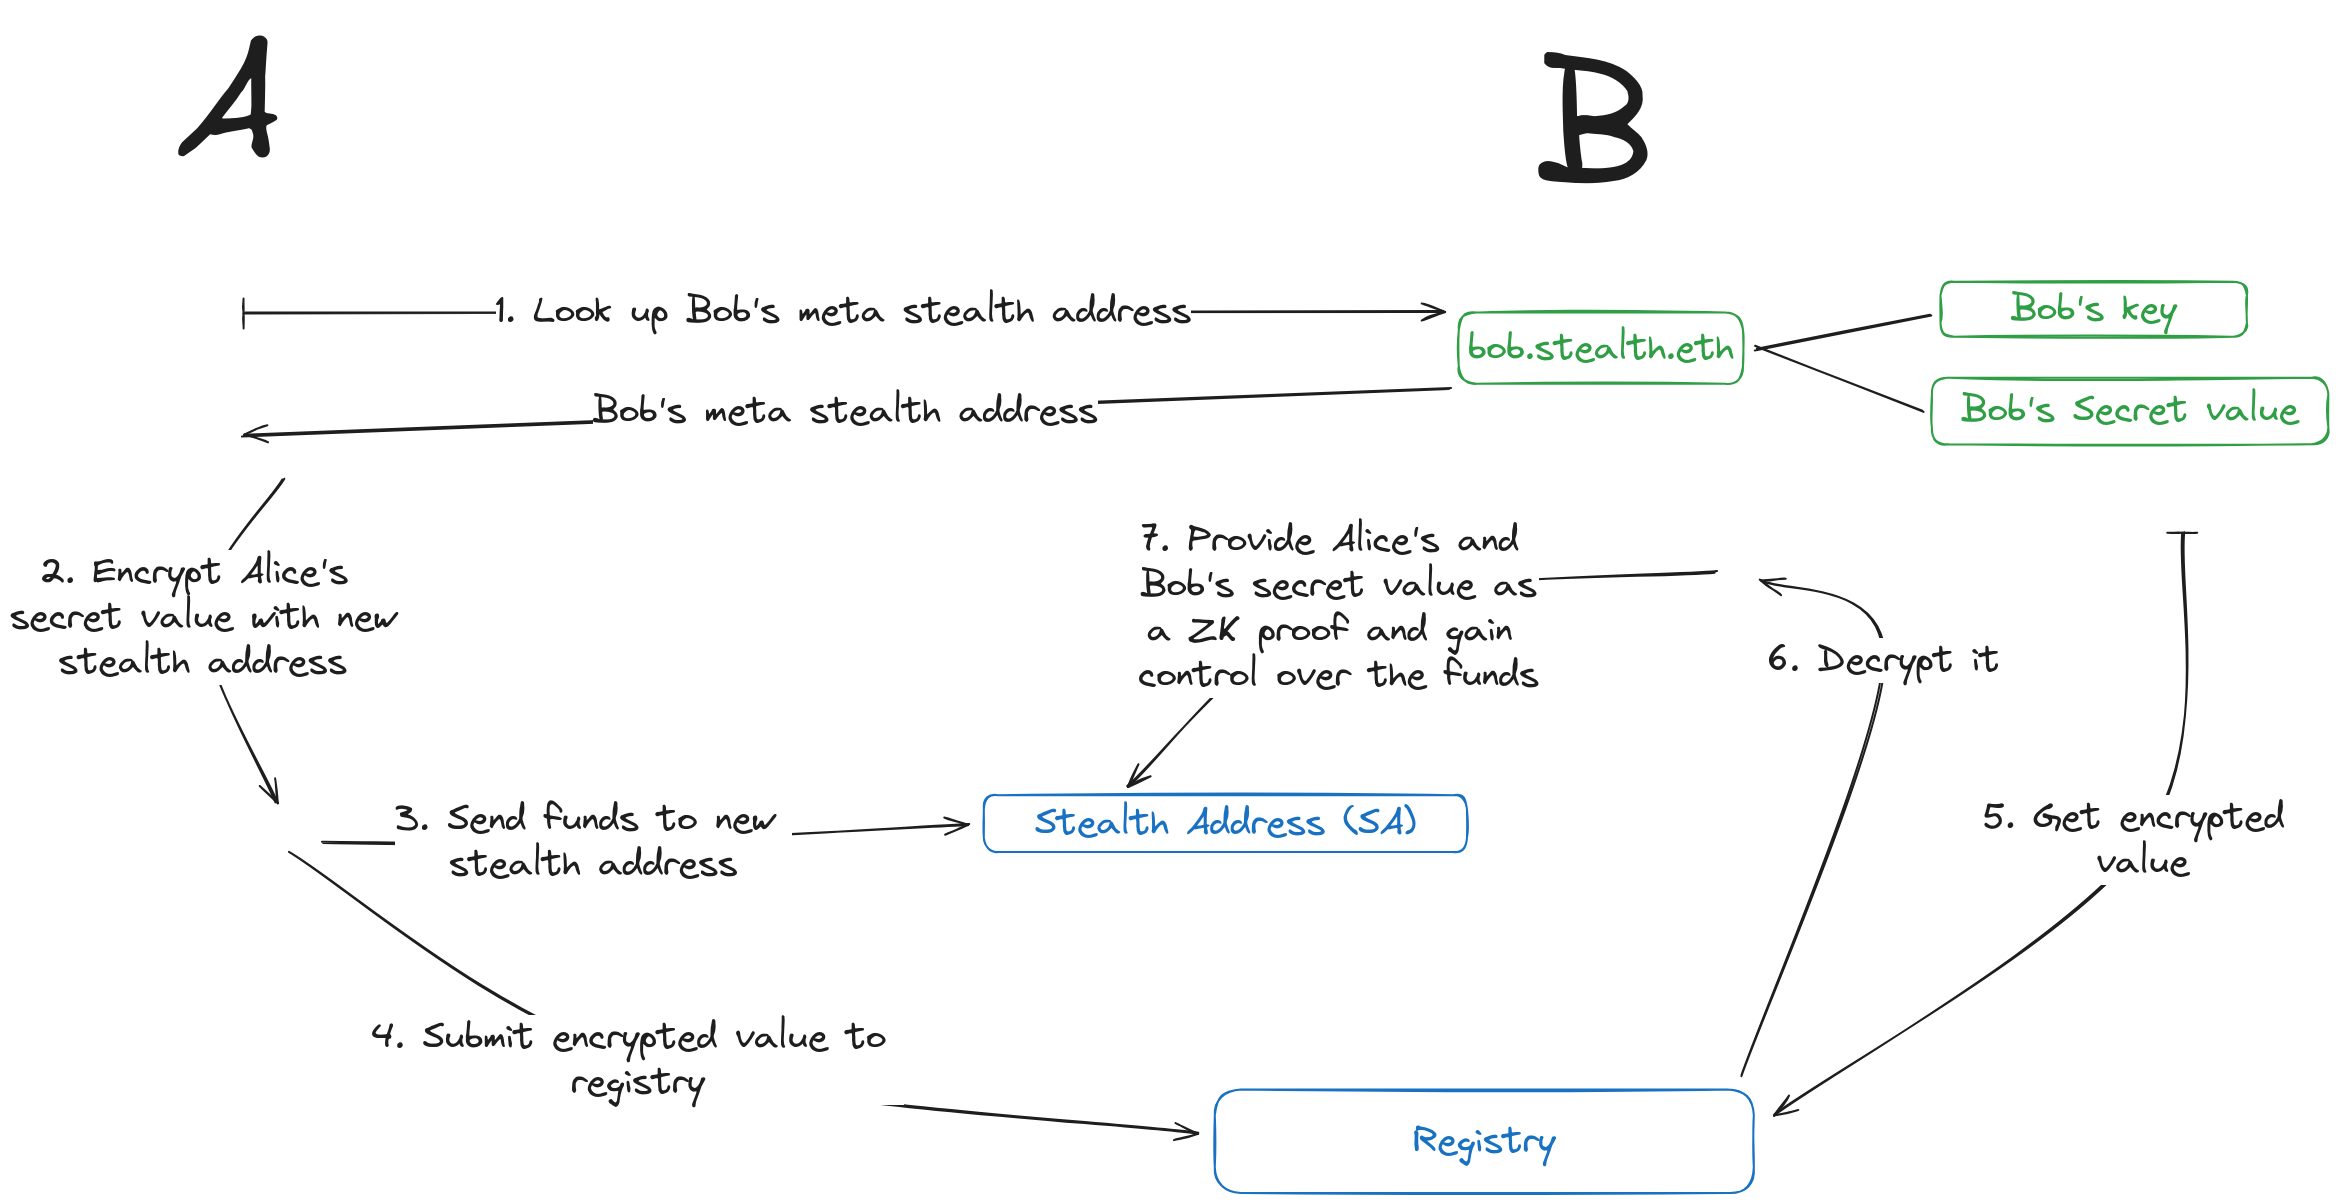
\includegraphics[scale=0.20]{assets/images/high-level.png}
    \caption{High Level Overview}
    \label{fig:hig-level}
	\cite{ButerinIncompleteGuide}
    \vspace{0.5cm}
\end{figure}

\section{Initial Setup}

Before Alice can send funds to Bob, Bob must first publish his meta stealth
address to some public location. Bob computes the following:

\begin{itemize}
	\item A private key $k$,
	\item A corresponding public key $K$,
	\item A secret value $x$,
	\item A hash of the secret value $h = hash(x)$.
\end{itemize}

Bob then publishes his meta stealth address in the form of a tuple $(K, h)$.
The hash is later used to prove to a stealth address contract that Bob is the
owner of the address and can spend funds sent to it.

\begin{figure}[h]
    \centering
    
\includegraphics[scale=0.30]{assets/images/initial-setup.png}
    \caption{Initial Setup}
    \label{fig:initial-setup}
	\cite{ButerinIncompleteGuide}
    \vspace{0.5cm}
\end{figure}

\section{Sending Funds}

When Alice wishes to send funds to Bob, she must first generate a new stealth
address. Alice looks up Bob's meta stealth address $(K, h)$ and computes the
following:

\begin{itemize}
	\item A secret value $c$,
	\item A new random stealth address $SA$,
	\item An ephemeral key $P = encrypt(value=[c, SA], key=K)$,
	\item A code $C = hash(h, c)$.
\end{itemize}

Alice then creates a smart contract at the new stealth address $SA$, which contains
the code $C$ and sends funds to it. Then in the same transaction, Alice sends
the ephemeral key $P$ to public registry contract, which stores the ephemeral
keys for all stealth addresses.

\begin{figure}[h]
    \centering
    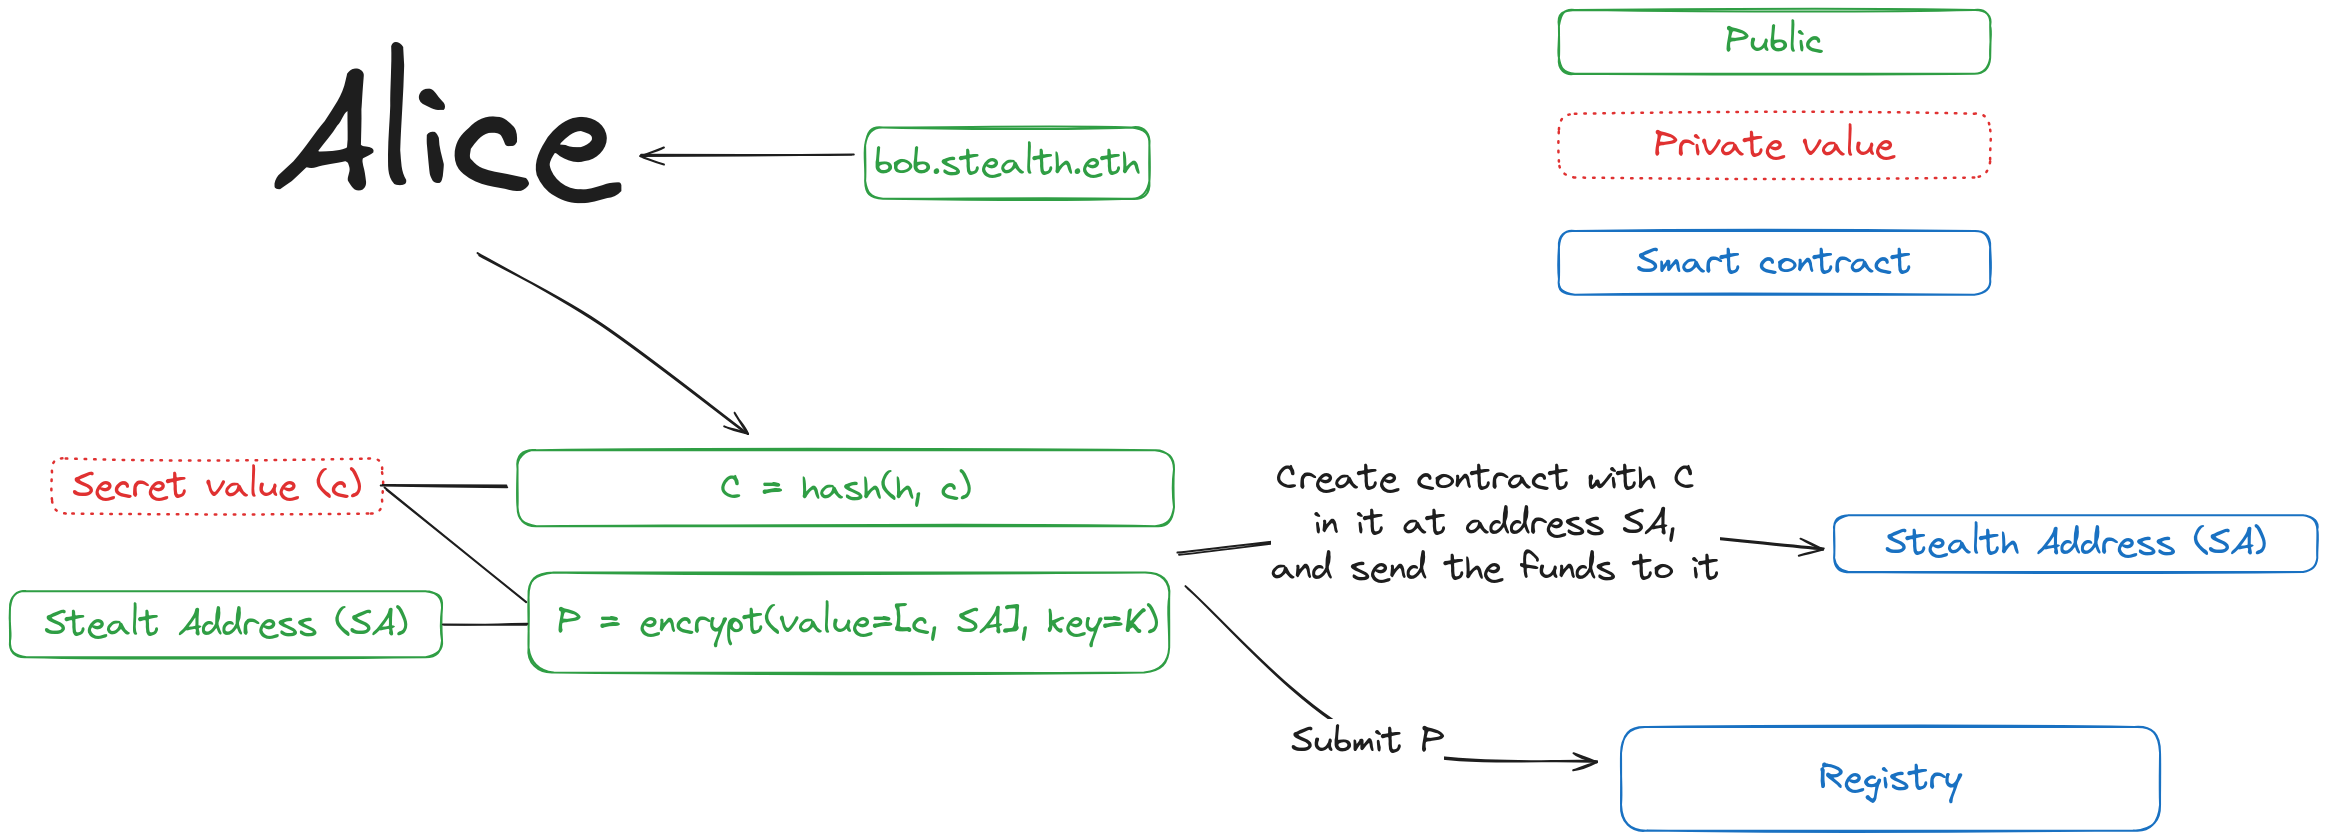
\includegraphics[scale=0.20]{assets/images/sending-funds.png}
    \caption{Sending Funds}
    \label{fig:sending-funds}
	\cite{ButerinIncompleteGuide}
    \vspace{0.5cm}
\end{figure}

\section{Scanning for Stealth Addresses}

Bob scans for stealth addresses by querying the public registry contract
from tha last point he scanned. The registry contract returns a list of
ephemeral keys. Bob then decrypts each ephemeral key with his private key $k$.
If the ephemeral key is meant for Bob, then it will contain the secret value
$c$ and the stealth address $SA$.

\section{Gaining control of Stealth Addresses}

Bob can gain control of the stealth address $SA$ by proving to the stealth
address contract that he is the owner of the values $x$ and $c$, such that\\
$C = hash(h, c) = hash(hash(x), c)$. Bob does this by computing a ZKP for 
this statement and sending it in a transaction from any address (preferably
not from any Bob's publicly known addresses) to the stealth address $SA$. The
$SA$ contract verifies the proof and if it isn't valid, the transaction is
rejected.

\section{Overview}

The whole solution design is illustrated in Figure \ref{fig:solution},
and was inspired by the work of Vitalik Buterin\cite{ButerinIncompleteGuide}.

\begin{figure}[h]
    \centering
    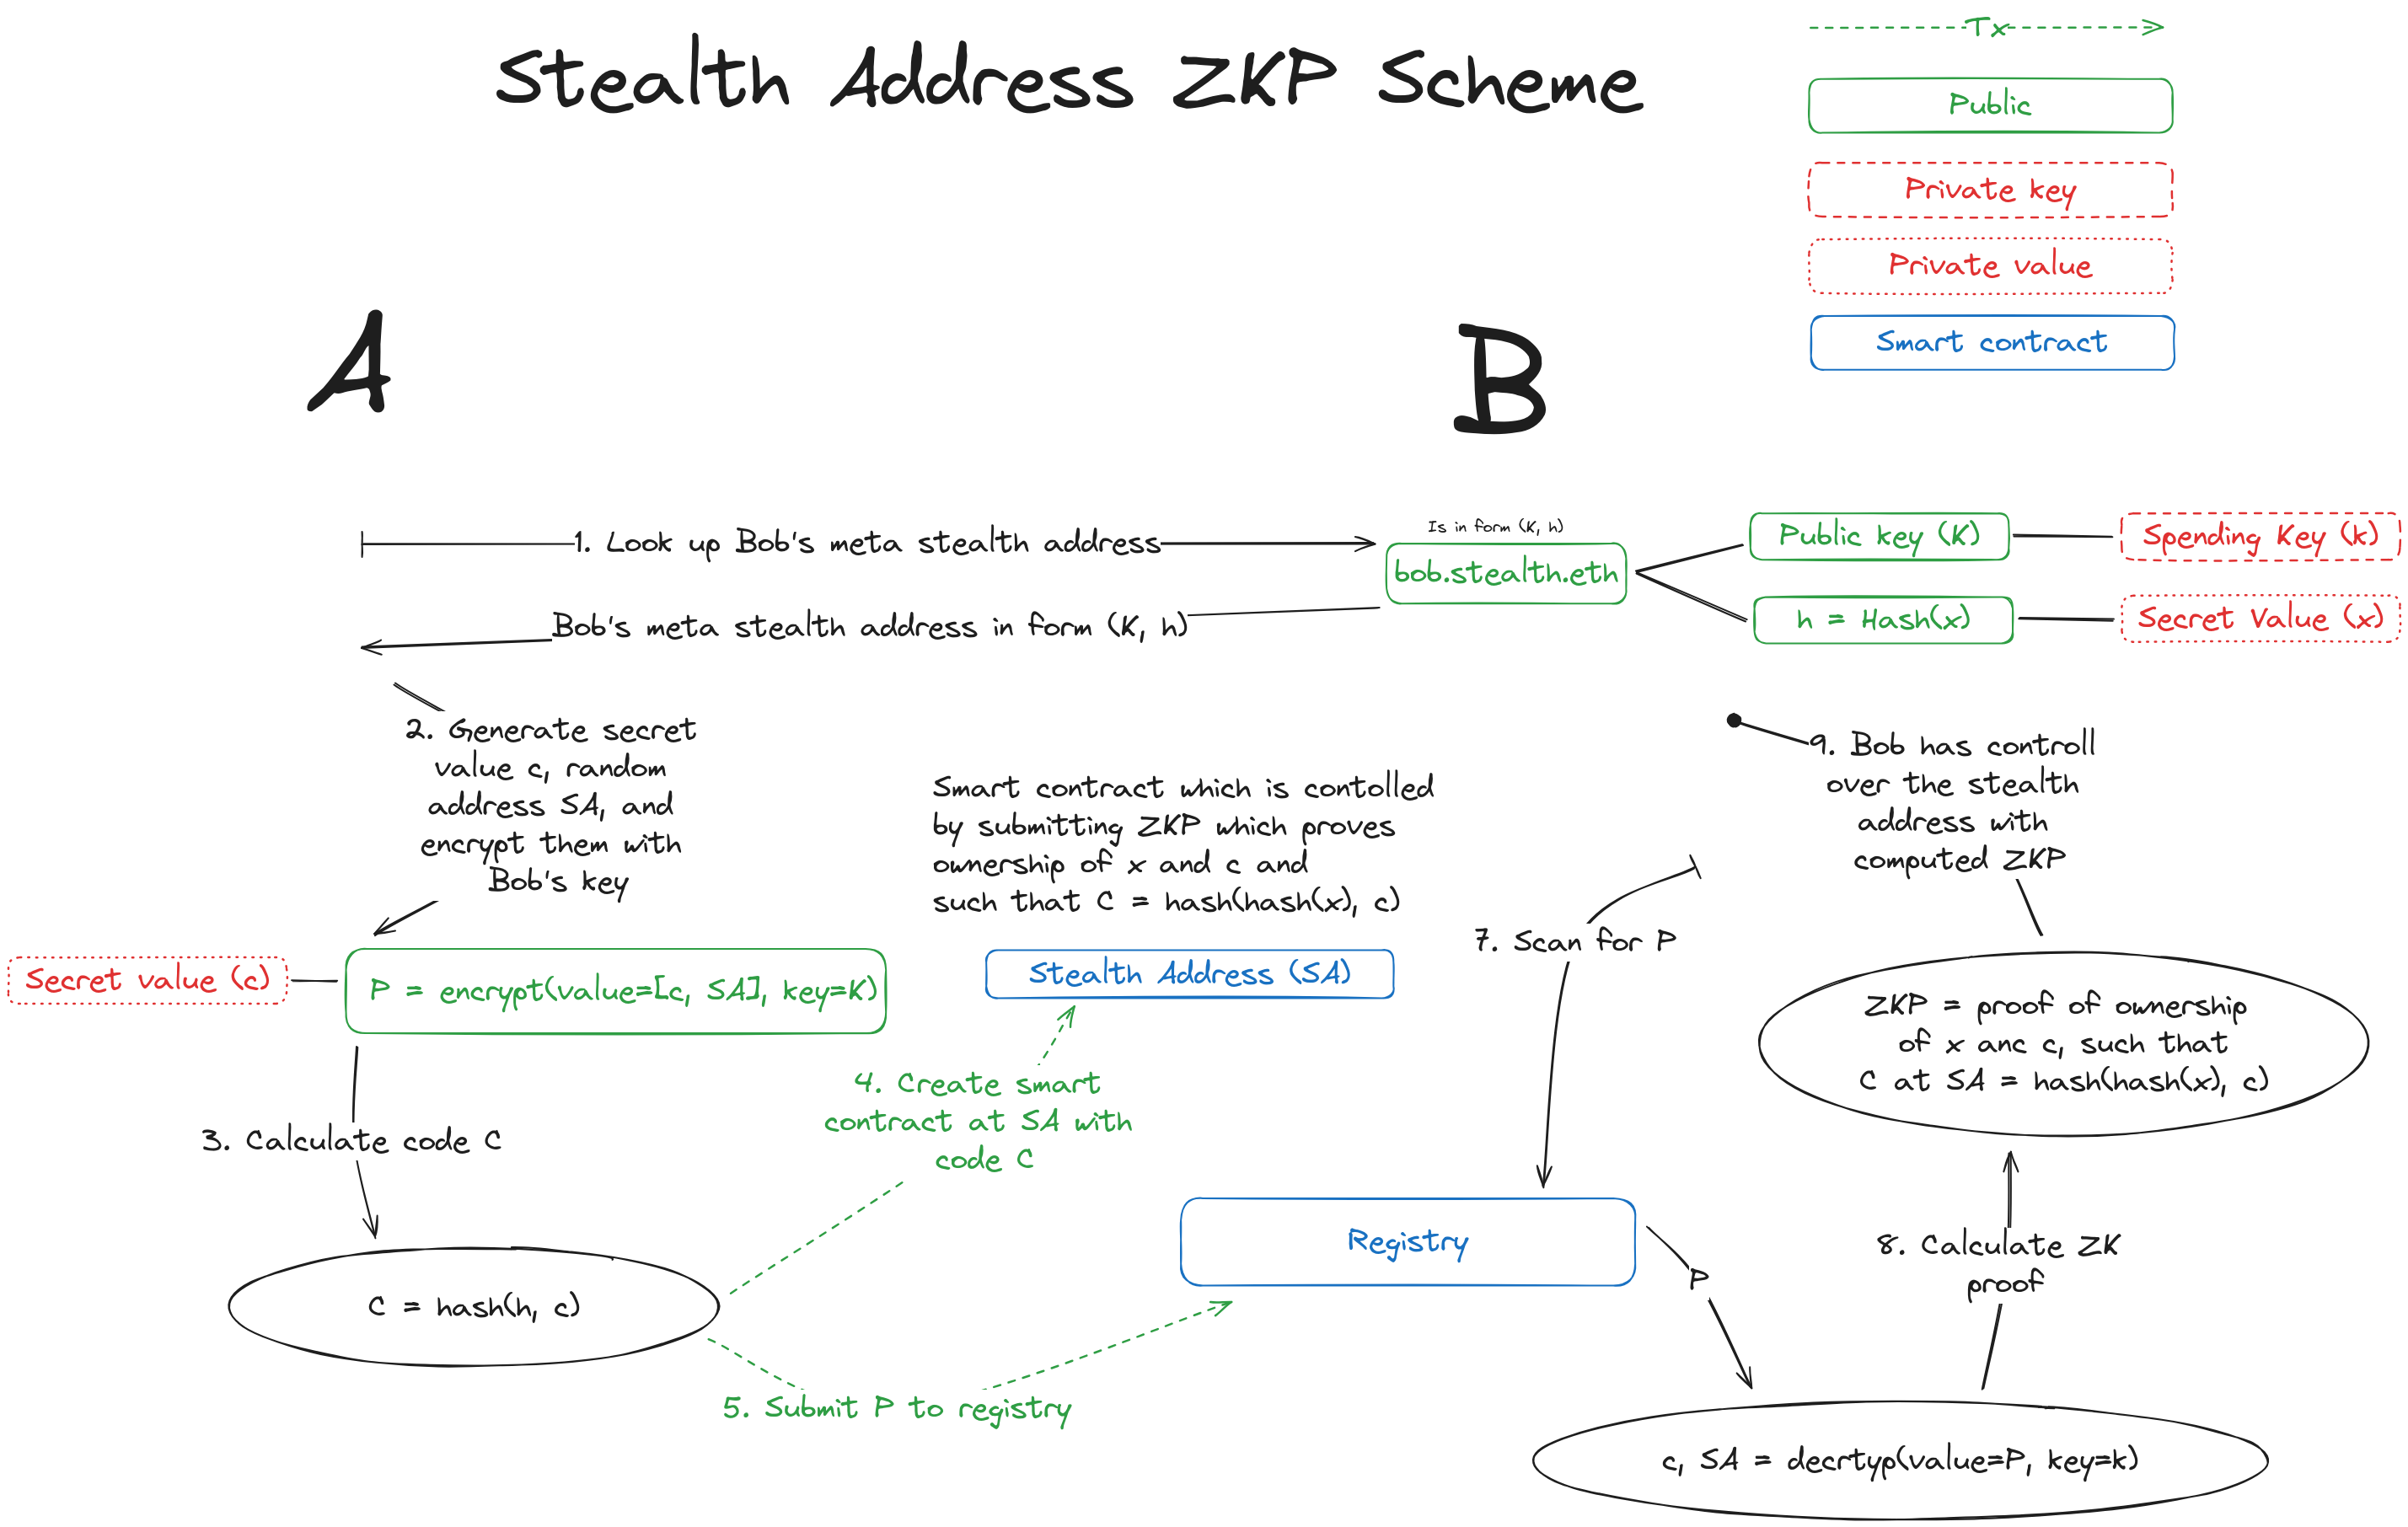
\includegraphics[scale=0.15]{assets/images/solution.png}
    \caption{Solution Design}
	\cite{ButerinIncompleteGuide}
    \label{fig:solution}
    \vspace{0.5cm}
\end{figure}



    \chapter{Discussion on security}

In this chapter, the security of the Stealth Address ZKP Scheme is informally discussed.

\section{Assumptions}

\subsection{Groth16}

It is assumed that the pairing-based ZK-SNARK system Groth16\cite{Groth16} has these properties:
\begin{enumerate}
    \item Completness - honest prover will always convince honest verifier
    \item Soundness - dishonest prover will not convince honest verifier
    \item Zero Knowledge - dishonest verifier will learn nothing more then the truth of the given proposition
\end{enumerate}

If the completness property would not hold, Bob could be locked out of his stealth
addresses, because he could not prove to them that he possessed both secrets.

If the soundness would not hold, adversary could forge a false proof, which
would be verified as true, and thus could gain access to Bob's assets on given
stealth address.

And finally, if the zero knowledge property would not hold, an adversary could
learn Bob's identity, hence it would no longer be a stealth address.

\subsection{Trusted Setup}

The setup phase of Groth16\cite{Groth16} includes a trusted setup in order to generate
public parameters. The premise of the trusted setup is that the original parameters
used to create the public ones are thrown away, if not then the party which
produced public parameters can forge false proofs, yet the verifier would
recognize them as valid ones.

In context of this work, if a party creating the circuit didn't delete the
original parameters, then it could prove malicious statements about ownership
of the secret values needed to gain control over any stealth address.

\subsection{Collision resistant hash function}\label{crhf}

First assumption is that, the used instantiation of a hash function (\textit{H})
is a collision resistant one. Meaning it is computationally hard to find two
inputs \textit{a}, \textit{b}, such that

\[ a \neq b \land H(a) = H(b) \]

Otherwise, an adversary could, for example, find a value $x^\prime$,
such that Bob's secret value $x$ and $x^\prime$ are not equal, but their hashes
are. Then the $x^\prime$ could be used to gain control over Bob's stealth address,
if the adversary knew Alice's secret value, or in the case when Alice is a malicious
actor, she could send assets to Bob's stealth address, but with $x^\prime$ and
her secret value, could withdraw them without any public proof that she did it.

As showcased earlier, this vulnerability alone is not enough to gain control
over Bob's stealth address, adversary also must know Alice's secret value to
gain control over a Bob's stealth address, but only the one she interacted with.

Also, if used hash function is not a collision resistant one, adversary still can not
discover the identity of Bob, or any of his other stealth addresses.

\subsection{Elliptic Curve Crypthography - Secp256k1}

Next assumption is that the Secp256k1 elliptic curve parameters used in Ethereum
and Bitcoin\cite{bitcoinSecp256k1Bitcoin} are well-chosen and do not contain any backdoors. Additionally, it is
assumed that advancements in cryptographic research and technology do not
compromise the security of Secp256k1.

If not, an adversary could recover Bob's private key and decrypt all of his
ephemeral keys submitted to the Ephemeral Key Registry contract. The
adversary would know all Bob's stealth addresses and, also have all secret
values used to create codes in those stealth addresses. However, with this
vulnerability alone, the adversary can not control Bob's stealth addresses,
because he/she is missing the Bob's secret value $x$.

\subsection{Knowledge of recipient's secret value}

If an adversary somehow learns Bob's secret value $x$, he/she does not have enough
information to control any of Bob's stealth addresses. On the other hand, if Alice,
or any other sender, would learn Bob's secret value $x$, she could, as in the
\ref{crhf} steal Bob's assets from the stealth address she interacted with and
Bob would not have any public proof that it was her.

\subsection{Knowledge of sender's secret value}

If an adversary somehow learns Alice's secret value $c$, the corresponding
address is still safe, because, the attacker does not know which stealth address
it is, and if somehow learned it, he/she still does not have Bob's secret value.

\section{Discussion summary}

Given these assumptions, the presented Stealth Address ZKP Scheme can be used to
send assets to a recipient, without leaking any information about him/her. And
guarantees to the recipient that only he/she has access to stealth addresses.



    \chapter{Implementation}\label{chapter:implementation}

In this section different terminology is used, instead of Bob, owner is used,
and instead of Alice sender is used. The implementation of this study is
separated into 3 modules (depicted in \ref{fig:component-diagram}), module for the
circuit which will compute ownership proofs, another one for smart contracts
needed to implement stealth wallet with ZKP stealth address schema, and
module with a web app wallet client used to interact with the stealth wallets.

The implementation is only a proof of concept, not a full featured wallet.
The sender's part is the same as described until now. The owner however,
can only withdraw all funds from the wallet into another address. This does
not detract from demonstrating the core concept of a ZKP stealth address schema.
Fractional withdrawals, ERC20 token transfers, transaction proxying and other wallet
features can be implemented in future work.

\begin{figure}[h!]
    \centering
    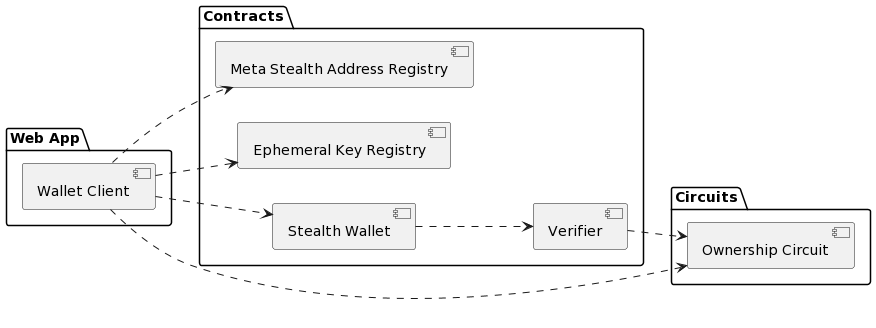
\includegraphics[width=\textwidth]{assets/images/component-diagram.png}
    \caption{Component diagram}
    \label{fig:component-diagram}
    \vspace{0.5cm}
\end{figure}

\section{Interaction between components}

The interaction between components, and users is depicted in Figure \ref{fig:component-diagram}.

\begin{figure}[h!]
    \centering
    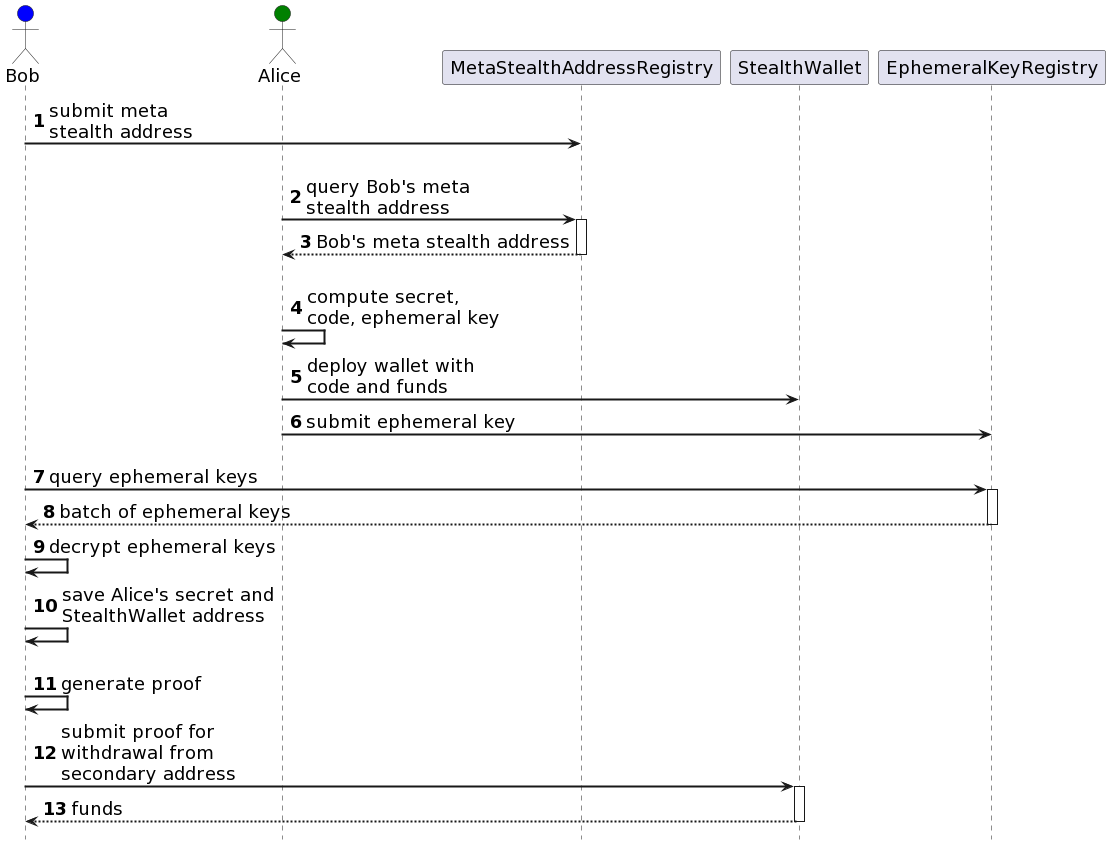
\includegraphics[width=\textwidth]{assets/images/implementation-flow.png}
    \caption{Component diagram}
    \label{fig:implementation-diagram}
    \vspace{0.5cm}
\end{figure}


\section{Circuits}

Circuits for proving and verifying ZKPs are written in Circom 2 \cite{circomCircomDocumentation}.
With circom compiler, a circuit is compiled into a Groth16
ZK-SNARK proof system \cite{Groth16} representation. Circom also generates
either C++ of Wasm source files for computing witness (proof) for the
circuit. Circuit written in this study, which proves ownership, has
these private inputs:
\begin{enumerate}
    \item owner's secret value,
    \item sender's secret value,
    \item and the withdrawee address.
\end{enumerate}
And these public inputs:
\begin{enumerate}
    \item code that was submitted by sender on contract creation,
    \item and the transaction sender.
\end{enumerate}

Groth16 requires a trusted setup for each circuit. For Groth16 trusted
setup, there are two parts:
\begin{enumerate}
    \item Powers of Tau ceremony \cite{PowersOfTau},
    \item and phase 2 dependent on the circuit.
\end{enumerate}
Powers of Tau ceremony is used to generate initial parameters for a SNARK.
In this ceremony, the initial parameters are generated using a multi-party
computation. If only one party in this computation is acting honestly,
the entire process is trustworthy and the initial parameters are secure
for use with any circuit. There is ongoing public powers of tau ceremony
called Perpetual Powers of Tau \cite{PerpetualPTAU}. Its goal is to
securely generate SNARK parameters for circuits. In this study a powers
of tau ceremony file from SnarkJS \cite{snarkjs} is used, which is from
this ceremony. Phase 2 is generated with SnarkJS and is specific for circuit.

\section{Smart contracts}

Smart contracts in this implementation are written in programming
language Solidity \cite{solidity} and are developed and tested
with Foundry \cite{foundry}. They are deployed through
Infura \cite{infura} Ethereum RPC provider to the Sepolia Ethereum
testnet \cite{sepolia}.

There are four smart contracts implemented. A meta stealth address
registry which holds meta stealth addresses. A ephemeral key registry
which holds the ephemeral keys. A verifier of previously mentioned
circuit. And contract for the stealth wallet.

Owners submit their meta stealth addresses to meta stealth address registry,
and senders query it for them. To the ephemeral key registry senders submit
ephemeral keys and owners query it for them. Senders deploy stealth wallets
with funds and computed codes. Owners send proofs to stealth wallets,
which interact with the verifier.

This module also contains tests. Code coverage report for these is shown in
table \ref{table:coverage}.

\begin{table}[ht]
\centering
\scalebox{0.7}{
    \begin{tabular}{l | r r r r}
    \toprule
        \textbf{File} & \textbf{\% Lines} & \textbf{\% Statements}  & \textbf{\% Branches}  & \textbf{\% Funcs} \\ 
        \midrule
        script/DeployConfig.s.sol  & 0.00\% (0/5)    & 0.00\% (0/7)     & 0.00\% (0/2)     & 0.00\% (0/3)   \\
        script/DeployContracts.s.sol & 0.00\% (0/7)    & 0.00\% (0/9)     & 100.00\% (0/0)   & 0.00\% (0/1)   \\
        src/EphemeralKeyRegistry.sol & 92.86\% (13/14) & 94.44\% (17/18)  & 66.67\% (4/6)    & 66.67\% (2/3)  \\
        src/MetaStealthAddressRegistry.sol & 100.00\% (8/8)  & 100.00\% (11/11) & 100.00\% (4/4)   & 100.00\% (2/2) \\ 
        src/StealthWallet.sol  & 91.67\% (11/12) & 92.31\% (12/13)  & 83.33\% (5/6)    & 66.67\% (2/3)  \\
        src/Verifier.sol   & 100.00\% (0/0)  & 100.00\% (0/0)   & 100.00\% (0/0)   & 100.00\% (1/1) \\
        \midrule
        \textbf{Total} & 69.57\% (32/46) & 68.97\% (40/58)  & 72.22\% (13/18)  & 53.85\% (7/13) \\
        \bottomrule
        \end{tabular}
}
\caption{Solidity code coverage}
\label{table:coverage}
\end{table}

The first two files are not covered, because they only contain simple logic
for deploying contracts and do not interfere in any functionality of the
implemented stealth address scheme.

\section{Web app}

Browser wallet client used to interact with stealth wallets is written in
frontend framework SolidJS \cite{solidjs}, with Web3JS \cite{web3js}
as the main library for interacting with blockchain, and Infura \cite{infura}
is used as a Ethereum RPC provider.

It consists of two sub-pages, one for sender (Alice), in which a sender
can query meta stealth addresses and deploy stealth wallets only accessible
by the owners of corresponding meta stealth addresses. And the second one,
for owners (Bob) which displays all stealth wallets with balance and enables
owners to withdraw funds from them by generating ZKPs.



    \chapter{Conclusion}

\section{Summary}

This thesis has presented how ZKPs can be applied to the problem of stealth
addresses in Ethereum. How one can receive payments without revealing their
identity, and do so without the need to actively communicate with the sender.

This proof of concept of a ZKP Stealth Address scheme on Ethereum allows
a sender to send funds to a recipient without any prior communication, and
without submitting any data, that links the sender with the recipient, to the blockchain.
And allows the recipient to prove that they are the intended recipient of the
funds, without revealing their identity, and without the need to actively
communicate with the sender.


\section{Future Work}

The design and implementation of the ZKP stealth address scheme serves only as
a proof of concept. For this scheme to be widely adopted, additional work is
required. This chapter outlines some of the potential future work that could be
done to improve the scheme.

\subsection*{Ephemeral Key Search}

The current implementation of the ZKP stealth address scheme requires that sender
submits the ephemeral public key to a registry. The registry is just a simple
storage that stores these keys in a list. This method does not scale well with
mass adoption. Each recipient would have to scan the entire list of keys to
check if any belong to them.

Current ERC-5564\cite{ethereumERC5564Stealth} proposal, which differs from
here proposed scheme mainly in the use of elliptic curve cryptography instead
of ZKPs, uses view tags to reduce the number of keys that need to be scanned.
Or, different approach, proposed by Xin Wang, Li Lin, Yao Wang \cite{Wang2023}
utilizes subgroup membership assumption related to factoring for faster key
search.

\subsection*{Recoverability}

The current implementation of the ZKP stealth address scheme does not allow for
possibility of funds recovery. This means that if the recipient loses their
private key, they will not be able to recover their funds.

One way to address this issue would be to use a private key recovery
mechanism, such as Shamir Backup. With this approach, the stealth address
scheme would not need to be modified, because the private key recovery would
be handled outside of the blockchain.

Different approach would be to modify the stealth address scheme to implement
a concept of a Social Recovery Wallet. These types of wallets enable user to
assign guardians to their wallet. Guardians are different accounts, for example
friends, mobile phone, hardware wallet or some kind of institution. The wallet
holds a public key to some user owned private key. Only this key can control
the wallet. If the user loses their private key, they can request the
guardians to change the associated public key in the wallet, thus changing the
private key that is used to control the wallet\cite{ButerinSocialRecovery}.
An incomplete implementation of this concept was proposed by Vitalik Buterin\cite{ButerinIncompleteGuide},
which uses ZKPs to prove to the stealth addresses, that the user is the owner
of the wallet.




    % \chapter{Future Work}

The design and implementation of the ZKP stealth address scheme serves only as
a proof of concept. For this scheme to be widely adopted, additional work is
required. This chapter outlines some of the potential future work that could be
done to improve the scheme.

\section{Ephemeral Key Search}

The current implementation of the ZKP stealth address scheme requires that sender
submits the ephemeral public key to a registry. The registry is just a simple
storage that stores these keys in a list. This method does not scale well with
mass adoption. Each recipient would have to scan the entire list of keys to
check if any belong to them.

Current ERC-5564\cite{ethereumERC5564Stealth} proposal, which differs from
here proposed scheme mainly in the use of elliptic curve cryptography instead
of ZKPs, uses view tags to reduce the number of keys that need to be scanned.
Or, different approach, proposed by Xin Wang, Li Lin, Yao Wang \cite{Wang2023}
utilizes subgroup membership assumption related to factoring for faster key
search.

\section{Recoverability}

The current implementation of the ZKP stealth address scheme does not allow for
possibility of funds recovery. This means that if the recipient loses their
private key, they will not be able to recover their funds.

One way to address this issue would be to use a private key recovery
mechanism, such as Shamir Backup. With this approach, the stealth address
scheme would not need to be modified, because the private key recovery would
be handled outside of the blockchain.

Different approach would be to modify the stealth address scheme to implement
a concept of a Social Recovery Wallet. These types of wallets enable user to
assign guardians to their wallet. Guardians are different accounts, for example
friends, mobile phone, hardware wallet or some kind of institution. The wallet
holds a public key to some user owned private key. Only this key can control
the wallet. If the user loses their private key, they can request the
guardians to change the associated public key in the wallet, thus changing the
private key that is used to control the wallet\cite{ButerinSocialRecovery}.
An incomplete implementation of this concept was proposed by Vitalik Buterin\cite{ButerinIncompleteGuide},
which uses ZKPs to prove to the stealth addresses, that the user is the owner
of the wallet.




    \ifx\FIITlagEN\undefined
    \else
        % Resume in Slovak
\thispagestyle{empty}

\begin{otherlanguage}{slovak}
\chapter*{Resumé}
\markboth{Resumé}{Resumé}
\addcontentsline{toc}{chapter}{Resumé} 

\end{otherlanguage}

    \fi

    % Bibliography
    \printbibliography[heading=references,segment=\therefsegment]

    % no page numbers for appendices
    \addtocontents{toc}{\protect\setcounter{tocdepth}{0}}
    \addtocontents{toc}{\cftpagenumbersoff{chapter}}

\end{refsegment}

% Appendix
\appendix

% Time schedule
\thispagestyle{empty}

\ifx\FIITlagEN\undefined
\chapter{Harmonogram práce}
\else
\chapter{Project task schedule}
\fi

\pagenumbering{arabic}
\renewcommand*{\thepage}{B-\arabic{page}}

\section{Zimný semester}

\begin{tabular}{|l||l|}
\hline
1\textsuperscript{st}-4\textsuperscript{th} week    & Consultations \& finding related research  \\
\hline
5\textsuperscript{th}-6\textsuperscript{th} week    & Working on the Introduction and Analysis chapters  \\
\hline
7\textsuperscript{th} week                          & Consultations  \\
\hline
8\textsuperscript{th}-10\textsuperscript{th} week   & Working on the Analysis chapters  \\
\hline
11\textsuperscript{th}-12\textsuperscript{th} week  & Working on the Solution proposal chapter \\
\hline
\end{tabular}

\section{Letný semester}

\begin{tabular}{|l||l|}
\hline
1\textsuperscript{st}-2\textsuperscript{nd} week    & Consultations \& designing API specification  \\
\hline
3\textsuperscript{rd}-6\textsuperscript{th} week    & Consultations \& implementation of back-end  \\
\hline
7\textsuperscript{th}-9\textsuperscript{th} week    & Implementation of server  \\
\hline
10\textsuperscript{th} week                         & Consultations \& implementation of front-end  \\
\hline
11\textsuperscript{th}-12\textsuperscript{th} week  & Finishing documentation \& solution testing  \\
\hline
\end{tabular}


% % Contents of the digital medium
\thispagestyle{empty}

\ifx\FIITlagEN\undefined
    \chapter{Obsah digitálneho média}
\else
    \chapter{Contents of the digital medium}
\fi

\pagenumbering{arabic}
\renewcommand*{\thepage}{C-\arabic{page}}

\ifx\FIITlagEN\undefined
    \par Evidenčné číslo práce v informačnom systéme: \FIITevidenceNumber
\else
    \par Registration number of the thesis in the information system: \FIITevidenceNumber
\fi

\ifx\FIITlagEN\undefined
    \par Obsah digitálnej časti práce (archív ZIP):
\else
    \par Contents of the digital medium (ZIP archive):
\fi

% \begin{minted}[linenos=false]{text}
% Folder                  Contents
% /bin                    binárne súbory umožňujúce ...
%     /service
%     /app
% /models                 modely opísané v práci
%     modelA
%     modelB
% /scripts
% /data                   dátové množiny použité na ...
% /praca-pdf              pdf verzia záverečnej práce
%     /praca.pdf          pdf hlavná časť záverečnej práce
%     /prilohy.pdf        pdf textové prílohy záverečnej práce

% \end{minted}

% only if digital medium contents exceed 1 GB
% \par Digitálna časť práce má veľkosť 3.75 GB, kvôli čomu je uložená v systéme G Suite for Education.


\ifx\FIITlagEN\undefined
    \par Názov odovzdaného archívu: \FIITArchiveName.
\else
    \par Name of the submitted archive: \FIITArchiveName.
\fi


\end{document}
